\documentclass{article}
\usepackage{../../../../format}
\usepackage{enumerate}
\usepackage{xcolor}
\usepackage{tikz}
\usepackage{fancyvrb}
\usepackage{hyperref}
\usepackage{minted}
\lhead{Programming Paradigms - Systems Programming}
\definecolor{links}{HTML}{2A1B81}
\hypersetup{colorlinks,linkcolor=,urlcolor=blue}
\usetikzlibrary{shapes.misc}
\usetikzlibrary{shapes.geometric, arrows, positioning}

\title{Systems Programming --- Lecture 5:\\
Memory Access using Pointers}
\author{Dr Konrad Dabrowski\\
\href{mailto://konrad.dabrowski@durham.ac.uk}{konrad.dabrowski@durham.ac.uk}
}
\date{E103 Christopherson Building\\
}

\begin{document}

\begin{center}
	\underline{\huge Memory Access using Pointers}
\end{center}

\section{Implementing variables}

\begin{defin}[Variable]
A logical name for an allocated area of memory assigned to store a value of a certain type	
\end{defin}


\begin{minted}{c}
int i = 10;
\end{minted}

\begin{center}
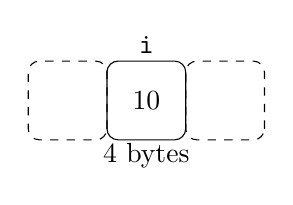
\begin{tikzpicture}
\draw[rounded corners, dashed] (2, 0) rectangle (1, 1) {};
\draw[rounded corners, dashed] (0, 0) rectangle (-1, 1) {};
\draw[rounded corners] (0, 0) rectangle (1, 1) {};
\node at (0.5,1.2) {\texttt{i}};
\node at (0.5,0.5) {$10$};
\node at (0.5,-0.2) {4 bytes};
\end{tikzpicture}
\end{center}




\section{Pointer variables}
\begin{center}
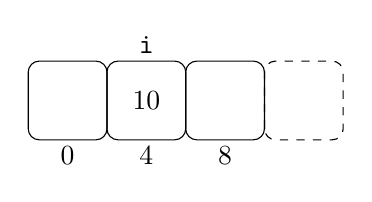
\begin{tikzpicture}
\begin{scope}[shift={(-1,0)}]
\draw[rounded corners] (0, 0) rectangle (1, 1) {};
\node at (0.5,-0.2) {$0$};
\end{scope}
\begin{scope}[shift={(1,0)}]
\draw[rounded corners] (0, 0) rectangle (1, 1) {};
\node at (0.5,-0.2) {$8$};
\end{scope}
\draw[rounded corners] (0, 0) rectangle (1, 1) {};
\node at (0.5,1.2) {\texttt{i}};
\node at (0.5,0.5) {$10$};
\node at (0.5,-0.2) {$4$};
\begin{scope}[shift={(2,0)}]
\draw[rounded corners,dashed] (0, 0) rectangle (1, 1) {};
\end{scope}
\end{tikzpicture}
\end{center}
\begin{itemize}
\item 
\begin{minted}{c}
int i = 10;
\end{minted}

\item value of \verb!i! is \verb!10!

\item The memory address of \verb!i! is \verb!&i! and has a value of \verb!4!

\item A pointer variable stores a memory address:
\begin{minted}{c}
int *p;
p = &i;      
\end{minted}
\item now the pointer variable \verb!p! stores the memory address of the integer variable \verb!i!
\end{itemize}




\section{Pointers}

\begin{center}
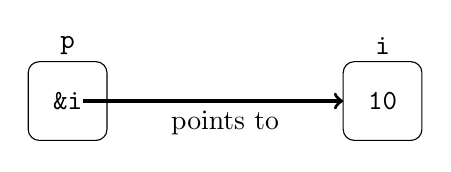
\begin{tikzpicture}
\draw[rounded corners] (0, 0) rectangle (1, 1) {};
\node at (0.5,1.2) {\texttt{i}};
\node at (0.5,0.5) {\texttt{10}};
\node[anchor=north] at (-1.5, 0.5) {points to};

\draw[rounded corners] (-4, 0) rectangle (-3, 1) {};
\draw[very thick,->] (-3.3,0.5) -- (0,0.5);
\node at (-3.5,1.2) {\texttt{p}};
\node at (-3.5,0.5) {\texttt{\&i}};
\end{tikzpicture}
\end{center}

\begin{minted}{c}
int i = 10;   // simple variable
int *p = &i;  // pointer variable
\end{minted}

\begin{itemize}
\item You can read the address operator \verb!&! as \emph{address of}
\end{itemize}
 
\begin{minted}{c}
printf("%d %d\n", i, *p ) ;
\end{minted}

\begin{itemize}
\item This outputs \verb!10 10!

\item You can read the indirection operator \verb!*! as \emph{value of}
\end{itemize}



\section{Basic pointer operations}
\begin{minted}{c}
int i = 5; // declare an int variable
int *p;    // declare a variable pointer to an int

p = &i;    // & "address of"
\end{minted}

\begin{itemize}
\item Use indirection operator \verb!*! to access and modify the value:
\end{itemize}
\begin{minted}{c}
*p = 7;      // assign value of 7 to i

*p = *p + 1; // add 1 to value of i
\end{minted}



\section{The Indirection Operator: what not to do}
\begin{itemize}
\item Applying the indirection operator to an uninitialized pointer variable causes undefined behaviour:
\begin{minted}{c}
  int *p;
  printf("%d", *p);   /*** WRONG ***/
\end{minted}


\item Assigning a value to \verb!*p! is particularly dangerous:
\begin{minted}{c}
  int *p;
  *p = 1;   /*** DANGER ***/
\end{minted}

\end{itemize}



\section{Pointer Assignment}
\begin{itemize}
\item C allows the use of the assignment operator to copy pointers of the same type

\item Assume that the following declaration is in effect:
\begin{minted}{c}
int i, j, *p, *q;
\end{minted}

\item Example of pointer assignment:
\begin{minted}{c}
p = &i;
\end{minted}
\end{itemize}

\begin{itemize}
\item Another example of pointer assignment:
\begin{minted}{c}
q = p;
\end{minted}
\item \verb!q! now points to the same place as \verb!p!:

\begin{center}
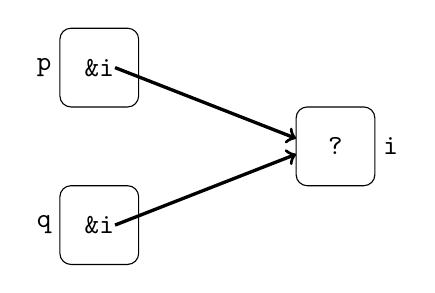
\begin{tikzpicture}
\draw[rounded corners] (-1, 0) rectangle (0, 1) {};
\node at (0.2,0.5) {\texttt{i}};
\node at (-0.5,0.5) {\texttt{?}};

\draw[rounded corners] (-4, 1) rectangle (-3, 2) {};
\draw[very thick,->] (-3.3,1.5) -- (-1,0.6);
\node at (-4.2,1.5) {\texttt{p}};
\node at (-3.5,1.5) {\texttt{\&i}};

\draw[rounded corners] (-4, -1) rectangle (-3, 0) {};
\draw[very thick,->] (-3.3,-0.5) -- (-1,0.4);
\node at (-4.2,-0.5) {\texttt{q}};
\node at (-3.5,-0.5) {\texttt{\&i}};
\end{tikzpicture}
\end{center}

\end{itemize}

\begin{itemize}
\item If \verb!p! and \verb!q! both point to \verb!i!, we can change \verb!i! by assigning a new value to either \verb!*p! or \verb!*q!:
\begin{minted}{c}
*p = 1;
\end{minted}

\begin{center}
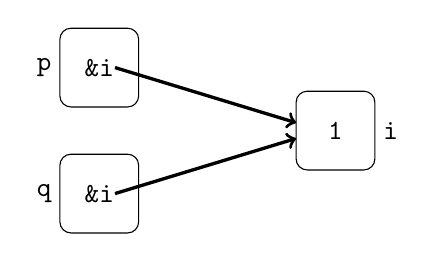
\begin{tikzpicture}
\draw[rounded corners] (-1, 0) rectangle (0, 1) {};
\node at (0.2,0.5) {\texttt{i}};
\node at (-0.5,0.5) {\texttt{1}};

\draw[rounded corners] (-4, 0.8) rectangle (-3, 1.8) {};
\draw[very thick,->] (-3.3,1.3) -- (-1,0.6);
\node at (-4.2,1.3) {\texttt{p}};
\node at (-3.5,1.3) {\texttt{\&i}};

\draw[rounded corners] (-4, 0.2) rectangle (-3, -0.8) {};
\draw[very thick,->] (-3.3,-0.3) -- (-1,0.4);
\node at (-4.2,-0.3) {\texttt{q}};
\node at (-3.5,-0.3) {\texttt{\&i}};
\end{tikzpicture}
\end{center}

\begin{minted}{c}
  *q = 2;
\end{minted}

\begin{center}
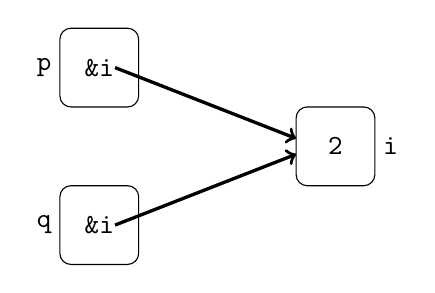
\begin{tikzpicture}
\draw[rounded corners] (-1, 0) rectangle (0, 1) {};
\node at (0.2,0.5) {\texttt{i}};
\node at (-0.5,0.5) {\texttt{2}};

\draw[rounded corners] (-4, 1) rectangle (-3, 2) {};
\draw[very thick,->] (-3.3,1.5) -- (-1,0.6);
\node at (-4.2,1.5) {\texttt{p}};
\node at (-3.5,1.5) {\texttt{\&i}};

\draw[rounded corners] (-4, -1) rectangle (-3, 0) {};
\draw[very thick,->] (-3.3,-0.5) -- (-1,0.4);
\node at (-4.2,-0.5) {\texttt{q}};
\node at (-3.5,-0.5) {\texttt{\&i}};
\end{tikzpicture}
\end{center}

\item Any number of pointer variables may point to the same object
\end{itemize}



\section{Pointers as Arguments}
\begin{itemize}
\item Previously we tried write a \verb!swap()! function that could modify its arguments, but it didn't work

\item By passing a pointer to a variable instead of the value of the variable, \verb!swap()! can be fixed
\end{itemize}



\section{Swap}
\begin{itemize}
\item We want to write a simple function in C to swap the values of two integer variables, \verb!x! and \verb!y!

\begin{minted}{c}
void swap(int a, int b) {
  int temp;
  
  temp = a;
  a = b;
  b = temp;
}
\end{minted}

\item Then call \verb!swap(x,y);!
\item Does this work?
\end{itemize}



\subsection{A working solution}
\begin{minted}{c}
void swap(int *a, int *b) {
  int temp;
  
  temp = *a;
  *a = *b;
  *b = temp;
}
\end{minted}

\begin{itemize}
\item Then call \verb!swap(&x,&y);!
\item Remember C uses call by value, but by using pointers you can get around this problem as the pointer still points at the original data
\end{itemize}



\section{Pointers as Arguments}
\begin{itemize}
\item Arguments in calls of \verb!scanf()! are pointers:

\begin{minted}{c}
  int i;
...
  scanf("%d", &i);
\end{minted}

\item Without the \verb!&!, \verb!scanf()! would be supplied with the value of \verb!i!

\item Although \verb!scanf()!'s arguments must be pointers, it's not always true that every argument needs the \verb!&! operator:
\begin{minted}{c}
  int i, *p;
...
  p = &i;
  scanf("%d", p);
\end{minted}

\item Using the \verb!&! operator in the call would be wrong:
\begin{minted}{c}
  scanf("%d", &p);   /*** WRONG, would be the address of the pointer,
   rather than the address of the thing p points at ***/
\end{minted}
\end{itemize}



\section{Arrays in C}
\begin{minted}{c}
int a[10];
\end{minted}

\begin{itemize}
\item declares a fixed size array holding ten \verb!int! values

\begin{center}
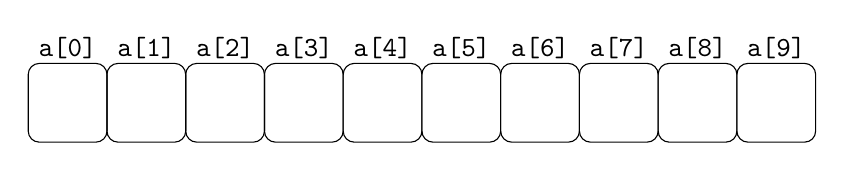
\begin{tikzpicture}
\begin{scope}[shift={(9,0)}]
\draw[rounded corners] (0, 0) rectangle (1, 1) {};
\node at (0.5,1.2) {\texttt{a[9]}};
\end{scope}
\begin{scope}[shift={(8,0)}]
\draw[rounded corners] (0, 0) rectangle (1, 1) {};
\node at (0.5,1.2) {\texttt{a[8]}};
\end{scope}
\begin{scope}[shift={(7,0)}]
\draw[rounded corners] (0, 0) rectangle (1, 1) {};
\node at (0.5,1.2) {\texttt{a[7]}};
\end{scope}
\begin{scope}[shift={(6,0)}]
\draw[rounded corners] (0, 0) rectangle (1, 1) {};
\node at (0.5,1.2) {\texttt{a[6]}};
\end{scope}
\begin{scope}[shift={(5,0)}]
\draw[rounded corners] (0, 0) rectangle (1, 1) {};
\node at (0.5,1.2) {\texttt{a[5]}};
\end{scope}
\begin{scope}[shift={(4,0)}]
\draw[rounded corners] (0, 0) rectangle (1, 1) {};
\node at (0.5,1.2) {\texttt{a[4]}};
\end{scope}
\begin{scope}[shift={(3,0)}]
\draw[rounded corners] (0, 0) rectangle (1, 1) {};
\node at (0.5,1.2) {\texttt{a[3]}};
\end{scope}
\begin{scope}[shift={(2,0)}]
\draw[rounded corners] (0, 0) rectangle (1, 1) {};
\node at (0.5,1.2) {\texttt{a[2]}};
\end{scope}
\begin{scope}[shift={(1,0)}]
\draw[rounded corners] (0, 0) rectangle (1, 1) {};
\node at (0.5,1.2) {\texttt{a[1]}};
\end{scope}
\draw[rounded corners] (0, 0) rectangle (1, 1) {};
\node at (0.5,1.2) {\texttt{a[0]}};
\end{tikzpicture}
\end{center}

\item \verb!a[i]! is the \verb!i!th element of the array
\item \verb!sizeof(a) = 10 * sizeof(int) = 40! bytes
\item The array is stored in memory as a single contiguous block that is 40 bytes (10 \verb!int!s) in size

\item Note that \verb!sizeof(a) / sizeof(a[0])=10!
\begin{itemize}
\item This is a common way of checking the number of elements in an array.
\item We can't pass an array to a function, but we can pass a pointer to it. The line above will not work correctly on a pointer, so we will need to pass the length of the array too.
\end{itemize}
\end{itemize}



\section{Strings}
\begin{itemize}
\item Are represented as an array of characters
\begin{minted}{c}
char a[] = "Hello worlds";
char b[13];
b = a; // Not allowed
char *c;
c = a;
\end{minted}
\item will set pointer \verb!c! to same address as \verb!a!
\item assignment of an array to array is not supported in C
\item unlike \verb!struct! as we saw last lecture
\item \verb!strcpy(b,a);!  first argument is the destination, ordered like assignment above
\begin{itemize}
\item need to \verb!#include<string.h>!
\end{itemize}
\end{itemize}




\begin{minted}{c}
char a[] = "Hello";
strlen(a) = 5; // number of characters
sizeof(a) = 6; // includes the null character at the end
\end{minted}

\begin{itemize}
\item Strings are null terminated -- important when allocating space to store them
\begin{minted}{c}
printf("%s %c\n", a, a[0]);
\end{minted}
\item Output is:
\begin{minted}{c}
Hello H
\end{minted}

\item If you use the variable \verb!a! on its own, it represents the memory address of the start of the string
\end{itemize}



\section{Pointers, strings and arrays}

\begin{center}
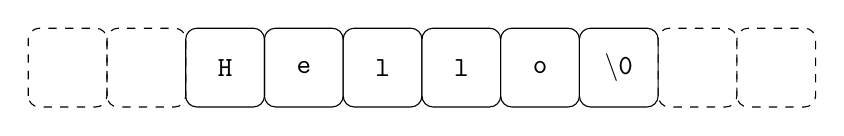
\begin{tikzpicture}
\begin{scope}[shift={(7,0)}]
\draw[rounded corners,dashed] (0, 0) rectangle (1, 1) {};
\end{scope}
\begin{scope}[shift={(6,0)}]
\draw[rounded corners,dashed] (0, 0) rectangle (1, 1) {};
\end{scope}
\begin{scope}[shift={(5,0)}]
\draw[rounded corners] (0, 0) rectangle (1, 1) {};
\node at (0.5,0.5) {\texttt{\textbackslash0}};
\end{scope}
\begin{scope}[shift={(4,0)}]
\draw[rounded corners] (0, 0) rectangle (1, 1) {};
\node at (0.5,0.5) {\texttt{o}};
\end{scope}
\begin{scope}[shift={(3,0)}]
\draw[rounded corners] (0, 0) rectangle (1, 1) {};
\node at (0.5,0.5) {\texttt{l}};
\end{scope}
\begin{scope}[shift={(2,0)}]
\draw[rounded corners] (0, 0) rectangle (1, 1) {};
\node at (0.5,0.5) {\texttt{l}};
\end{scope}
\begin{scope}[shift={(1,0)}]
\draw[rounded corners] (0, 0) rectangle (1, 1) {};
\node at (0.5,0.5) {\texttt{e}};
\end{scope}
\draw[rounded corners] (0, 0) rectangle (1, 1) {};
\node at (0.5,0.5) {\texttt{H}};
\begin{scope}[shift={(-1,0)}]
\draw[rounded corners,dashed] (0, 0) rectangle (1, 1) {};
\end{scope}
\begin{scope}[shift={(-2,0)}]
\draw[rounded corners,dashed] (0, 0) rectangle (1, 1) {};
\end{scope}
\end{tikzpicture}
\end{center}

\begin{minted}{c}
char a[] = "Hello"; // sizeof = 6
char *a = "Hello"; // sizeof = 8  as pointers take 8 bytes
\end{minted}

\begin{itemize}
\item These are equivalent declarations, and create the identical bytes in memory, as shown above.
\item \emph{Warning:} using \verb!sizeof(a)! will give \verb!6! in the first case (the size of the array) and \verb!8! in the second case (the size of the pointer).\
\item In the second case, the string \verb!"Hello"! is constant and cannot be modified.
\item Pointers and arrays are often used interchangeably
\end{itemize}



\section{Pointer arithmetic}
\begin{itemize}
\item Pointer arithmetic accounts for the base type of the items: 

\begin{minted}{c}
int a[10];
int *pa;

pa = &a[0];
pa = a;
\end{minted}

\begin{center}
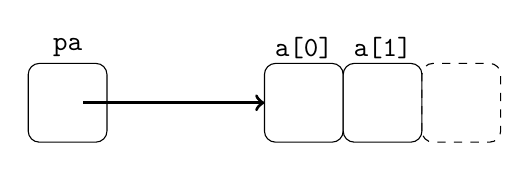
\begin{tikzpicture}
\draw[rounded corners] (0, 0) rectangle (1, 1) {};
\draw[rounded corners] (1, 0) rectangle (2, 1) {};
\draw[rounded corners,dashed] (2, 0) rectangle (3, 1) {};
\node at (0.5,1.2) {\texttt{a[0]}};
\node at (1.5,1.2) {\texttt{a[1]}};

\draw[rounded corners] (-3, 0) rectangle (-2, 1) {};
\draw[very thick,->] (-2.3,0.5) -- (0,0.5);
\node at (-2.5,1.2) {\texttt{pa}};
\end{tikzpicture}
\end{center}

\begin{minted}{c}
pa = &a[1];
pa = (a+1);
\end{minted}

\begin{center}
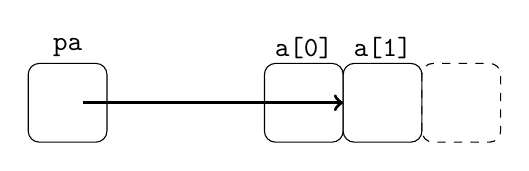
\begin{tikzpicture}
\draw[rounded corners] (0, 0) rectangle (1, 1) {};
\draw[rounded corners] (1, 0) rectangle (2, 1) {};
\draw[rounded corners,dashed] (2, 0) rectangle (3, 1) {};
\node at (0.5,1.2) {\texttt{a[0]}};
\node at (1.5,1.2) {\texttt{a[1]}};

\draw[rounded corners] (-3, 0) rectangle (-2, 1) {};
\draw[very thick,->] (-2.3,0.5) -- (1,0.5);
\node at (-2.5,1.2) {\texttt{pa}};
\end{tikzpicture}
\end{center}

\item The two pairs of statements above are equivalent using array or pointer notation: \verb!+1! translates to \verb!+4! bytes (1 \verb!int!)
\end{itemize}


% He stopped here
\section{Strange but true}
\begin{itemize}
\item In C if I write \verb!a[x]! this works by adding \verb!x! to \verb!a! to find the pointer
\item Hence \verb!a[x]! is the same as \verb!*(a+x)!
\item This seems fine if I write \verb!a[2]!
\item But what if I write \verb!2[a]!?
\item It compiles and works!
\item See \verb!array.c!
\end{itemize}



\section{What about?}
\begin{itemize}
\item \verb!a[-4]! ?
\item Interpreted as \verb!*(a + -4)!

\item Is the following valid?
\begin{minted}{c}
int *p;
int i = 5;
int j = 20;
p = &i;
printf("%d %d\n", p[0], p[1]);
\end{minted}

\item What will the output be?
\end{itemize}



\section{Peeking at memory}
\begin{itemize}
\item Can look at bits of memory
\item See \verb!peek.c!
\item Can find adjacent local variables and parameters
\item Easy to make mistakes
\item Cannot tell what data is by looking at it
\end{itemize}



\section{Breaking things}
\begin{itemize}
\item We can use random numbers to write random values in random places
\item See \verb!break.c!
\item This can upset the system
\item Segmentation fault occurs: hardware tells OS a memory access is not allowed
\item Sometimes it goes on for a shockingly long time
\item Sometimes the last number is very strange: why?
\end{itemize}




\end{document}

